\subsection{Overview}
The TrackMe services are built on a client-server structure, this way the system is organized through abstraction levels.
We chose to adopt a 3-tier architecture:
\begin{itemize}
	\item \textbf{Presentation Tier} \\This layer makes the interaction possible between the user and the system. Here the user sees all the information provided by the system in a easily way to understand them.
	\item \textbf{Application Tier} \\This layer is managed almost totally by Data4Help service that is in charge of:
	\begin{itemize}
		\item store data incoming from the external;
		\item collect data information from database in order to execute Third parties’ requests;
		\item also generates data statistics on data collected;
		\item send to third parties requested data.
	\end{itemize}
	Moreover even AutomatedSOS has logic application in order to continuously monitor users’ health status.
	\item \textbf{Data Tier} \\In this layer all the sensible users’ data (location, health status) are stored into Databases and are retrieved by the application tier in order to do statistics and answer third parties’ requests.
\end{itemize}

More specifically Data4Help manage the data and core logic sections while AutomatedSOS and Track4Run manage the presentation section. Actually, a small part of application tier is also present in AutomatedSOS, this is due to the fact that the Health Monitoring process requires to be executed as fast as possible.

\subsection{Component View}

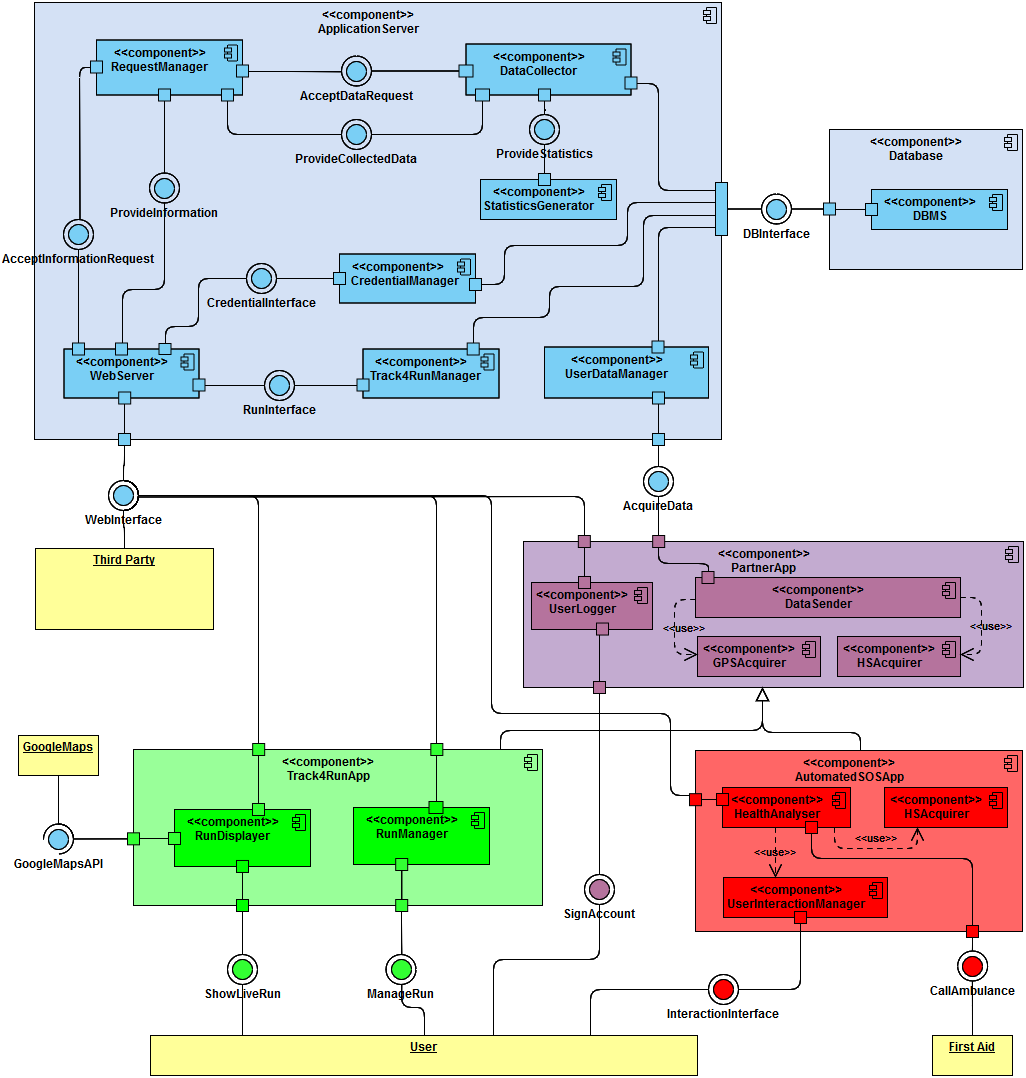
\includegraphics[scale=0.5]{Images/ComponentDiagram.png}

{\large \textbf{Component diagram description}}
\begin{enumerate}
\item [1] \textbf{Main Server} 
This huge component is in charge of manage Data4Help services so store and provide, for interested companies, users’ data (such as GPS location and daily Health Status). Moreover it manages race information of Track4Run application.

	\begin{enumerate}
	\item [1.1] \textbf{Web Server:} In order to accept and supply information to who need them, this component offer a friendly web interface to simplify these operations\\Offered interfaces:
		\begin{enumerate}
		\item [1.1.1] \textbf{Web Interface:} Human interface for third parties and Track4Run users. Software interface for AutomatedSOS.
		\item [1.1.2] \textbf{Web Interface:} Human interface for logging third parties.
		\end{enumerate}
		
	\item [1.2] \textbf{Request Manager:} In order to support web server in its job, this component manage all the incoming request: it sorts them per urgency, it wrap the request in a smart data structure and send it to Data Collector, it unwrap the answer from Data Collector and it continuously generates data exchange if a live acquisition is active\\Offered interfaces:
		\begin{enumerate}
		\item [1.2.1] \textbf{Accept Information request:} Software interface for Web server to allow receiving request to be evaluated.
		\item [1.2.2] \textbf{Offer Information:} Software interface for Web server to provide information answer.
		\end{enumerate}	
		
	\item [1.3] \textbf{Data Collector:} This component is in charge to communicate with Database in order to retrieve information and supply them to Request Manager. To perform these operations the component should receive request from Request Manger, unwrap it, creates a query to database that cover the question and send it to database; once the database has responded it should wrap the answer and provide it to Request Manager. Moreover if a statistic on data is required it requires it to Statistic Generator.\\Offered interfaces:
		\begin{enumerate}
		\item [1.3.1] \textbf{Accept request:} Software interface that accept request from Request manager formatted in the proper way.
		\item [1.3.2] \textbf{Provide managed data:} Software interface that provide to Request Manager information answer formatted in the proper way.
		\end{enumerate}	
		
	\item [1.4] \textbf{Statistic Generator:} This component is in charge of generates statistic on data provided by data collector such as arithmetic mean, variance from average, standard deviation and median.\\Offered interfaces:
		\begin{enumerate}
		\item [1.4.1] \textbf{Provide Statistics:} Software interface that provides statistic values to data collector.
		\item [1.4.2] \textbf{Provide Statistics:} (The Software interface to receive data from Data collector to be managed is trivial and not explicitly specified).
		\end{enumerate}	
	
	\item [1.5] \textbf{Users' Manager:} This component is in charge to communicate with users' device in order to log (or sign up) user and retrieve data collected.\\Offered interfaces:
		\begin{enumerate}
		\item [1.5.1] \textbf{Acquire Data:} Software interface that allows partner application to send data to Data4Help.
		\item [1.5.2] \textbf{Enroll user:} Software interface that allows user to become user of Data4Help service.
		\end{enumerate}	
	
	\item [1.6] \textbf{Track4Run Manager:} This component is in charge to communicate with Track4Run applications in order to allow promoter to manage races.\\Offered interfaces:
		\begin{enumerate}
		\item [1.6.1] \textbf{Acquire Data:} Software interface that allows promoter, through Track4Run, to promote a run, invite athletes and specify all the useful information about the race.
		\end{enumerate}	
	
	\end{enumerate}
	
\item [2] \textbf{Database} 
This component is in charge of store physically data and organize them in a smart way according to DBMS rule, moreover it allows the access to those data.

	\begin{enumerate}
	\item [2.1]\textbf{Users’ data DBMS:}
	This component is in charge of store all the users’ acquired data and quickly provide them to Data collector whenever it is required.\\Offered Interfaces:
		\begin{enumerate}
		\item [2.1.1] \textbf{Store users' Data:} Software interface that allows to Users’ data Acquirer to store data with queries.
		\item [2.1.2] \textbf{Retrieve Data:} Software interface that allows to Data Collector to collect data with queries.
		\end{enumerate}	
	
	\item [2.2]\textbf{Track4Run DBMS:}
	This component is in charge of store all the races' informations provided by promoters.\\Offered Interfaces:
		\begin{enumerate}
		\item [2.2.1] \textbf{Store races' Data:} Software interface that allows to Track4Run Manager to store data with queries.
		\item [2.2.2] \textbf{Retrieve Data:} Software interface that allows to Data Collector to collect data with queries.
		\end{enumerate}	
	
	\end{enumerate}

\end{enumerate}


\subsection{Deployment View}
The following Deployment Diagram captures the topology of the system's hardware.
The SmartphoneApp and SmartWatchApp (Presentation Tier) communicate to the Application Server through RMI, while the WebBrowser communicates to the WebServer through HTTP protocol. The Application Server (Application Tier) communicates to the Database Server (Data Tier) through JDBC.

\begin{figure}[H]
\centering
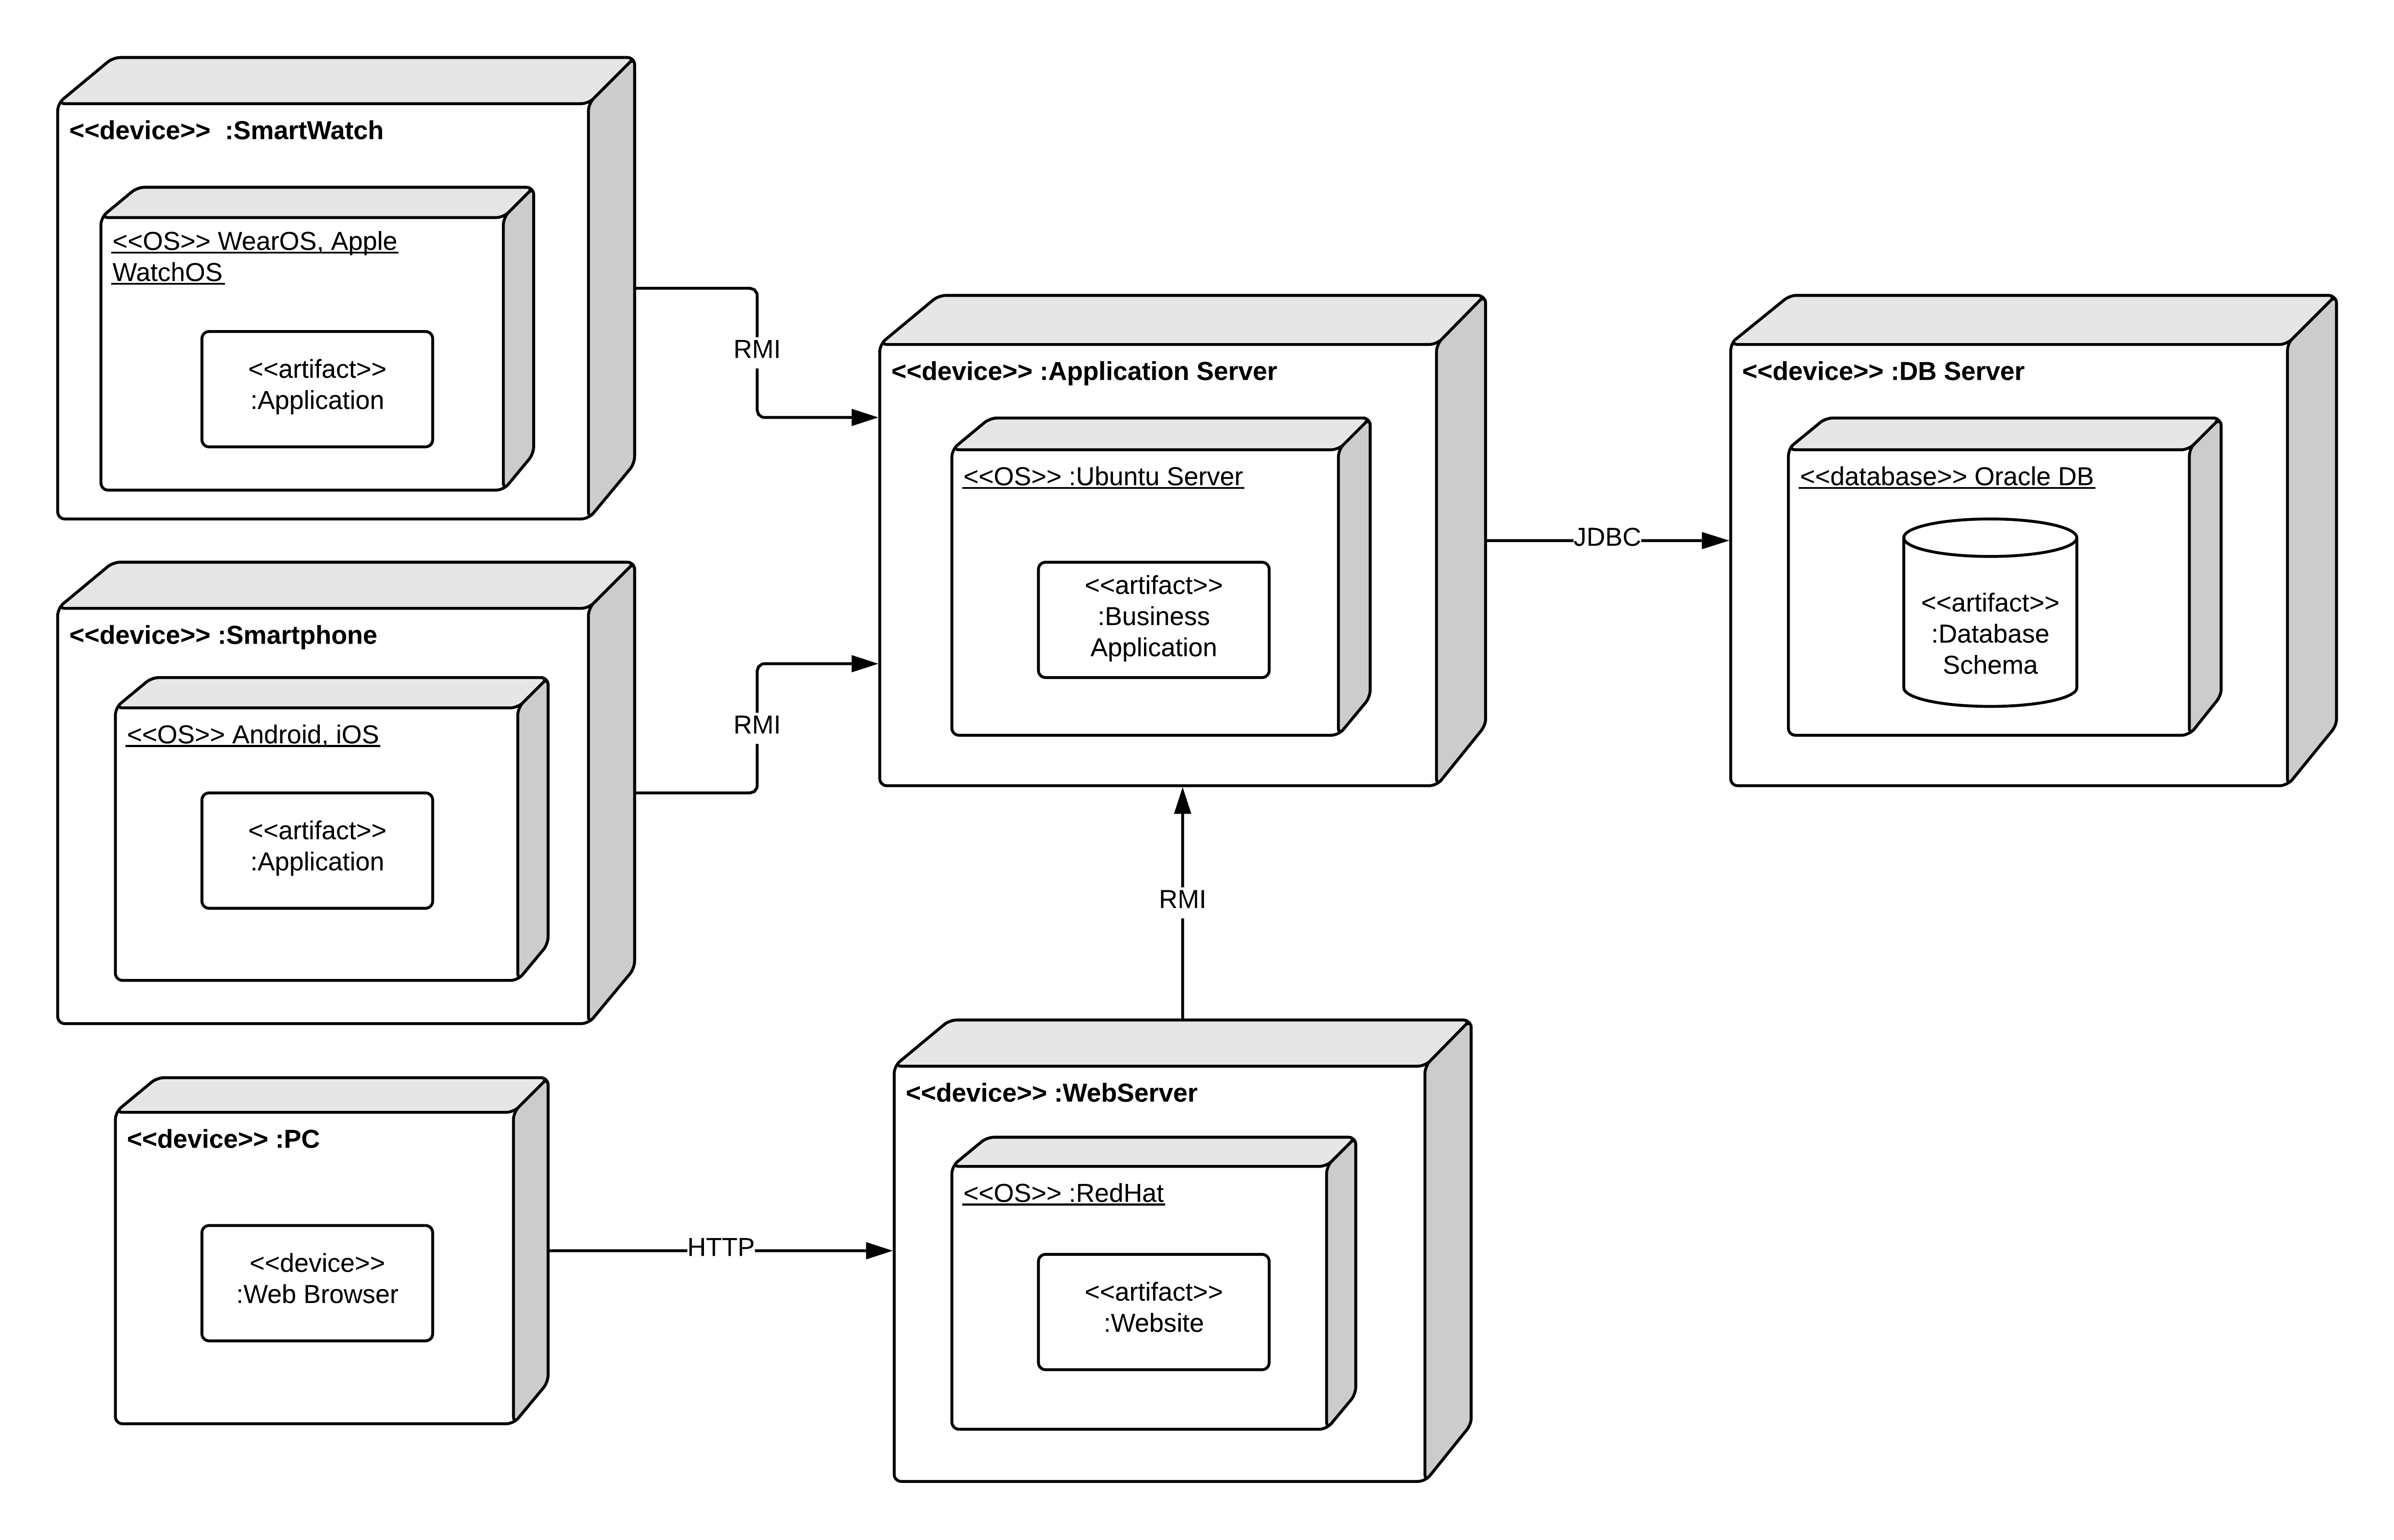
\includegraphics[scale=0.35]{Images/DeploymentDiagram.png}
\caption{Deployment Diagram.}
\end{figure}

\subsection{Runtime View}
In this section several Sequence Diagrams are shown in order to point up the interaction among components and their behavior in particular scenarios.

\subsubsection{Individual Request}

\subsubsection{}
\subsubsection{}


\subsection{Component Interfaces}
\subsection{Selected Architectural Styles and Patterns}
\subsection{Other Design Decisions}